\documentclass[conference]{IEEEtran}
\IEEEoverridecommandlockouts
% The preceding line is only needed to identify funding in the first footnote. If that is unneeded, please comment it out.
%Template version as of 6/27/2024

\usepackage{amsmath,amssymb,amsfonts}
\usepackage{algorithmic}
\usepackage{graphicx}
\usepackage{textcomp}
\usepackage{xcolor}
\usepackage[backend=biber,style=numeric]{biblatex}
\addbibresource{report.bib} 

 \graphicspath{{assets/latex/}}

\begin{document}

\title{CS6524 Computer Vision Lab. 1\\ Silhouettes and Fourier Epicycles}

\author{\IEEEauthorblockN{1\textsuperscript{st} Dawid Jakubowski}
\IEEEauthorblockA{\textit{ISE} \\
\textit{University of Limerick}\\
Limerick, Ireland \\
23384549@studentmail.ul.ie}
\and
\IEEEauthorblockN{2\textsuperscript{nd} Given Name Surname}
\IEEEauthorblockA{\textit{dept. name of organization (of Aff.)} \\
\textit{name of organization (of Aff.)}\\
City, Country \\
email address or ORCID}
\and
\IEEEauthorblockN{2\textsuperscript{nd} Given Name Surname}
\IEEEauthorblockA{\textit{dept. name of organization (of Aff.)} \\
\textit{name of organization (of Aff.)}\\
City, Country \\
email address or ORCID}
}

\maketitle

\section{Introduction}
This document explains the image transformations conducted. It explains the methodology, justification and discussion for each transformation. 

\section{Methodology}
\subsection{Grayscale}
\subsection{Blurring}
\subsection{Thresholding}
Binary thresholding was applied to the grayscale image to separate the foreground object from the background. The function accepts a 2D NumPy array and compares each pixel's intensity against a fixed threshold of 240. Pixels greater than or equal to the threshold are assigned 255 (white), while the remaining pixels are assigned 0 (black). The resulting binary image is returned as a NumPy array of type `uint8` for further processing.

\subsection{Border Detection}


\section{Justification}
\subsection{Grayscale}
\subsection{Blurring}
\subsection{Thresholding}
A fixed threshold of 127 was initially selected because it is approximately the midpoint of the 8-bit grayscale intensity range (0–255), however after testing this with various images we decided to change this value to 240 because our images had white backgrounds. NumPy's "np.where()" was used to apply the threshold across the entire image without explicit loops. The output was converted to `uint8` to maintain compatibility with other image-processing operations while minimizing memory usage.

\subsection{Border Detection}


\section{Discussion and failure analysis}
\subsection{Grayscale}
\subsection{Blurring}
\subsection{Thresholding}
Thresholding successfully converted the grayscale image into a binary representation. However, testing revealed that for our initial threshold value of 127, aspects of the foreground objects with similar intensities to the background were detected as the background (i.e. white).

\subsection{Border Detection}


\subsection{Lists}

List can be bulleted\dots
\begin{itemize}
\item First
\item Second
\item Third
\end{itemize}

Or enumerated

\begin{enumerate}
\item First
\item Second
\item Third
\end{enumerate}

\subsection{Equations}

Equations can have their own environment,
\begin{equation}
a+b=\gamma\label{eq}
\end{equation}
and be reference (Equation~\ref{eq}), or can be inline and blend in the text like this: $\sum_{i=0}^{N}x_i$, like any other word.

\subsection{Figures and Tables}

\begin{table}
\caption{Table Type Styles}
\begin{center}
\begin{tabular}{|c|c|c|c|}
\hline
\textbf{Table}&\multicolumn{3}{|c|}{\textbf{Table Column Head}} \\
\cline{2-4} 
\textbf{Head} & \textbf{\textit{Table column subhead}}& \textbf{\textit{Subhead}}& \textbf{\textit{Subhead}} \\
\hline
copy& More table copy$^{\mathrm{a}}$& &  \\
\hline
\multicolumn{4}{l}{$^{\mathrm{a}}$Sample of a Table footnote.}
\end{tabular}
\label{tab1}
\end{center}
\end{table}

\begin{figure}
% Uncomment the line below to include an image from a source file
\centerline{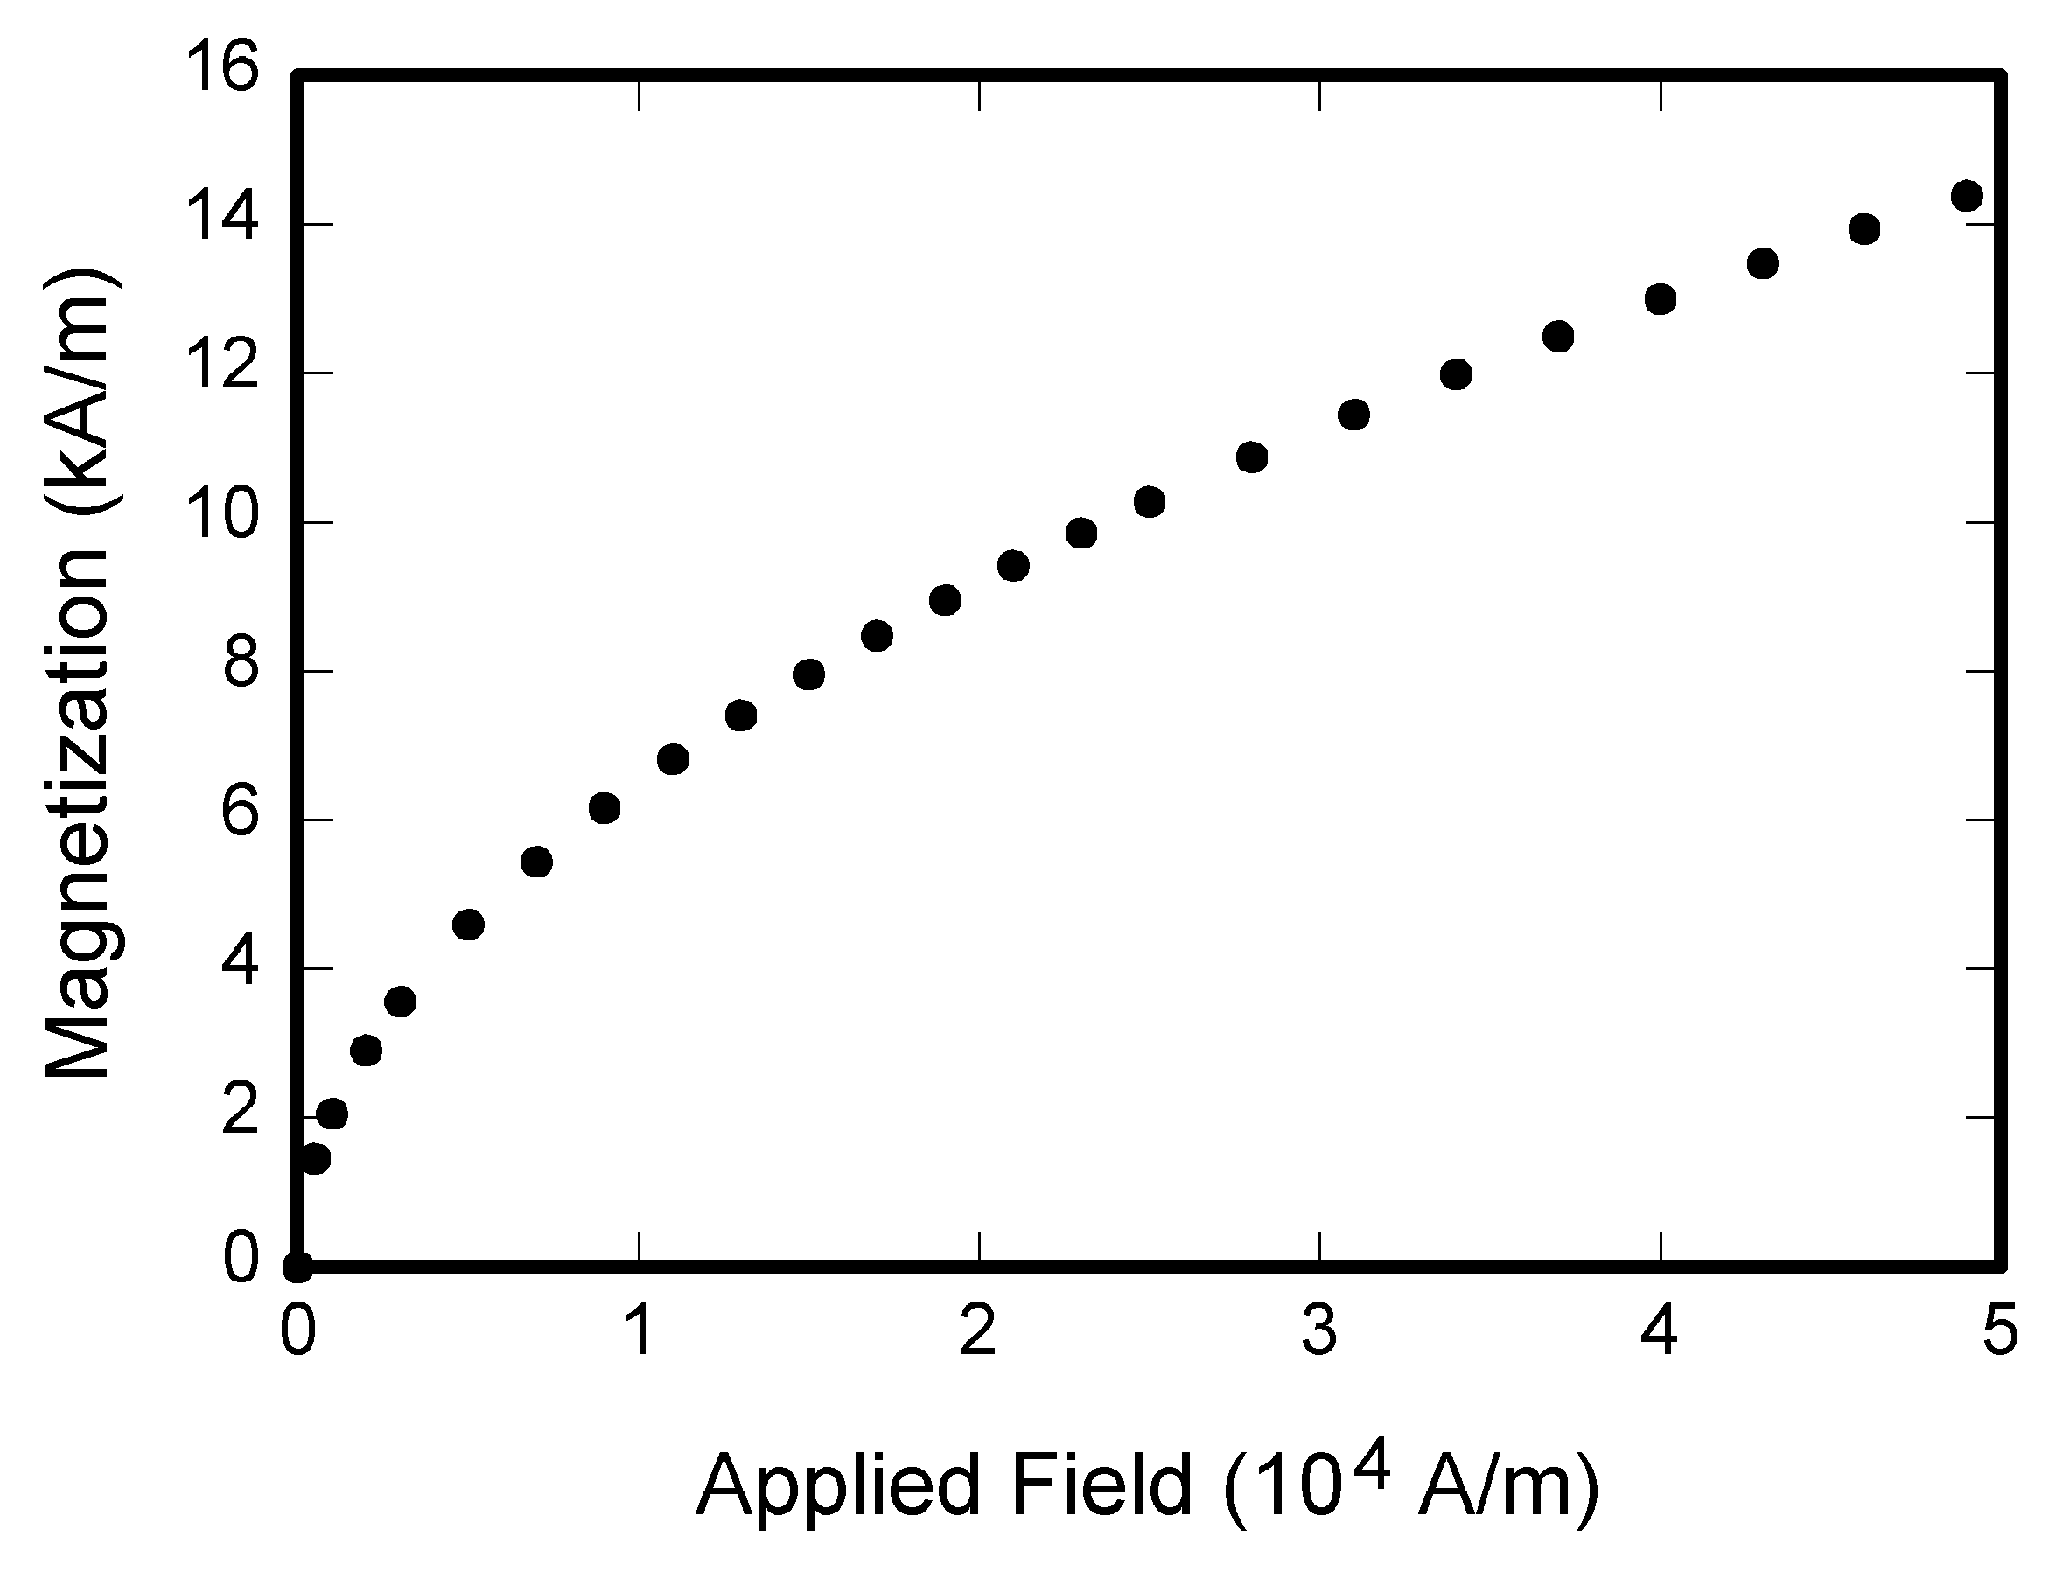
\includegraphics{fig1.png}}
\caption{Example of a figure caption.}
\label{fig}
\end{figure}

They appear by default on top of the text, and you reference like this: Figure~\ref{fig} and Table~\ref{tab1}.

\subsection{Citations}

If you need to cite external sources, use the \texttt{report.bib} file. As an example, here's how you cite the textbook~\cite{foundationsCVbook}.

\printbibliography

\end{document}